% -*- root: ../main.tex -*-
%!TEX root = ../main.tex
% vim:textwidth=120 fo=cqt

\frontmatter
\pagenumbering{arabic} % Imperial College requirement is that all pages must be in continuous arabic numbering
\graphicspath{{frontmatter/figures/}}


% Title page
% \pdfbookmark[chapter]{Title Page}{coverpage}

\includepdf[link, linkname=coverpage, addtotoc={1,chapter,0,Title Page,coverpage}, pages=-, pagecommand={\thispagestyle{plain}}]{frontmatter/coverpage.pdf}

% -*- root: ../main.tex -*-
%!TEX root = ../main.tex
% vim:textwidth=80 fo=cqt

\cleardoublepage

\newpage\null\thispagestyle{plain}\AddToShipoutPictureBG*{%
    \put(0,545){%
        \transparent{0.4}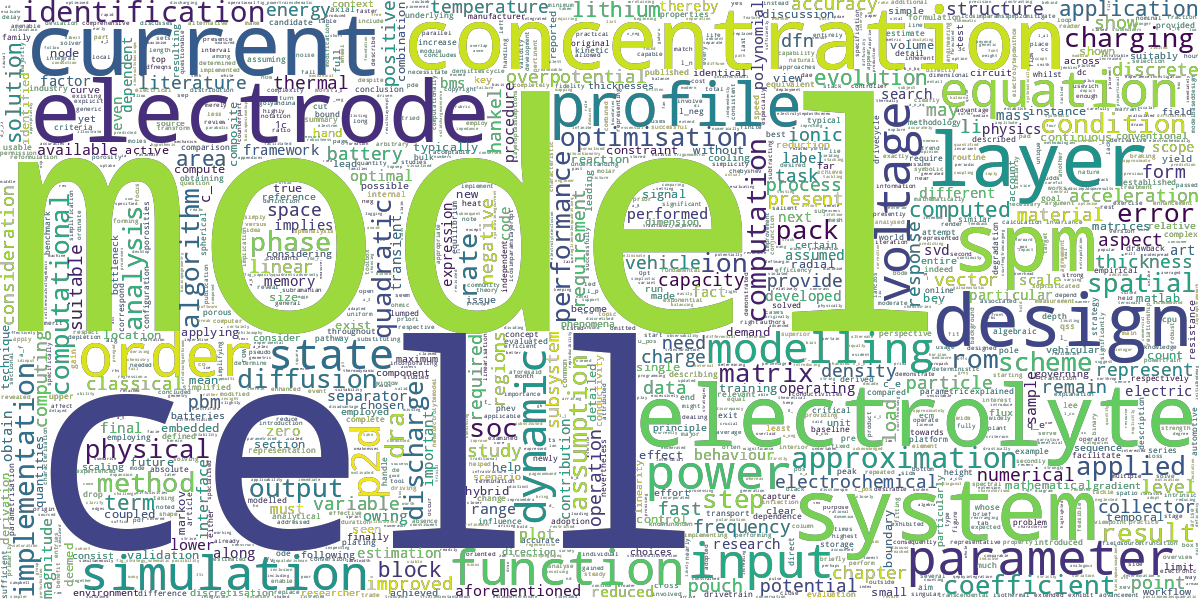
\includegraphics[width=\paperwidth,keepaspectratio]{wordcloud}%
    }%
}
\vfill
% \begin{minipage}[t]{105mm}
\parbox{130mm}{
    \doublespacing
    \noindent The professional biographical profile of this thesis author is available online at
    \url{https://www.linkedin.com/in/krishnakumargopalakrishnan/}
}
% \end{minipage}
% \begin{varwidth}[t]{10mm}
    \blackurl
    \qrcode[height=0.5in]{https://www.linkedin.com/in/krishnakumargopalakrishnan/}
    \regularurl
% \end{varwidth}
\newpage


% -*- root: ../main.tex -*-
%!TEX root = ../main.tex
% vim:textwidth=80 fo=cqt

% \pdfbookmark[chapter]{Originality \& Copyright Declarations}{} 

\chapter*{Declaration of Originality \hfill}\label{ch:originality}
\addcontentsline{toc}{chapter}{Declaration of Originality and Copyright}

\vspace*{-1.0cm}

I declare  that the material presented  in this thesis  is the result of  my own
research except  for specific portions wherein  contributions from collaborators
are acknowledged. Throughout this thesis, references are made to other published
works and  these have been appropriately  cited. The material contained  in this
thesis has  not been  submitted, either  in whole or  in part,  for a  degree at
Imperial College London or any other university.\\[-3em]

\begin{flushright}
        \begin{tabular}{@{}p{.4in}p{2.1in}@{}}
            % & 
\includegraphics[angle=-5,width=0.25\textwidth]{black_ink_sign_from_jpg}\\[-2em]
            % Signed: & \hrulefill \\
                    & \phantom{Krishnakumar Gopalakrishnan} \\
                    & Krishnakumar Gopalakrishnan \\
                    & October 02, 2018\\
                    & London, United Kingdom \\
        \end{tabular}
\end{flushright}

{\let\clearpage\relax \chapter*{Declaration of Copyright\hfill}}

\vspace*{-1cm}

\noindent
\begin{minipage}[b]{0.3275\textwidth}
    % https://www.imperial.ac.uk/research-and-innovation/support-for-staff/scholarly-communication/open-access/spiral/licences-and-policies/
    % newer link % https://www.imperial.ac.uk/research-and-innovation/support-for-staff/scholarly-communication/open-access/theses/selecting-a-creative-commons-licence/
    \noindent \raggedright 
\includegraphics[width=\linewidth]{doclicense-CC-by-nc-nd.pdf}
\end{minipage}
\hfill
\hspace*{0.0225\textwidth}
\begin{minipage}[b]{0.65\textwidth}
    The    copyright    of    this     thesis    rests    with    the    author.
    Unless   otherwise    indicated,   its    contents   are    licensed   under
    a   \href{https://creativecommons.org/licenses/by-nc-nd/4.0/}{\mbox{Creative
    Commons}   Attribution-NonCommercial-NoDerivatives  4.0   International  (CC
    BY-NC-ND 4.0) Licence}.
\end{minipage}

\noindent Under this licence, you may  copy and redistribute the material in any
medium or format on the condition that: you credit the author, do not use it for
commercial purposes  and do not distribute  modified versions of the  work. When
reusing or sharing this work, ensure you  make the licence terms clear to others
by naming  the licence and linking  to the licence text.  Please seek permission
from the copyright  holder for uses of  this work that are not  included in this
licence or permitted under UK Copyright Law.

\vfill


% -*- root: ../main.tex -*-
%!TEX root = ../main.tex
% vim:textwidth=80 fo=cqt

% \afterpage{\null\thispagestyle{plain}\newpage}

\chapter{Dedication\hfill}
% \addcontentsline{toc}{chapter}{Dedication}
\pagecolor{cornsilk}\afterpage{\nopagecolor}

\begingroup
\eachpageornament

\begin{minipage}{\textwidth}
    \vspace*{-2cm}
    \textcolor{black}{\heartpar{To my dear wife, \mbox{Parvathy C.S.}\ and my parents,
            \mbox{Gopalakrishnan P.K.} \& \mbox{Ananthalakshmi G}. The sacrifices that you all made for
            my success is immeasurable and no amount of words shall convey my sheer
    gratitude. I am forever in your debt for your unconditional love. }}

    \vfill
    \centering
    % 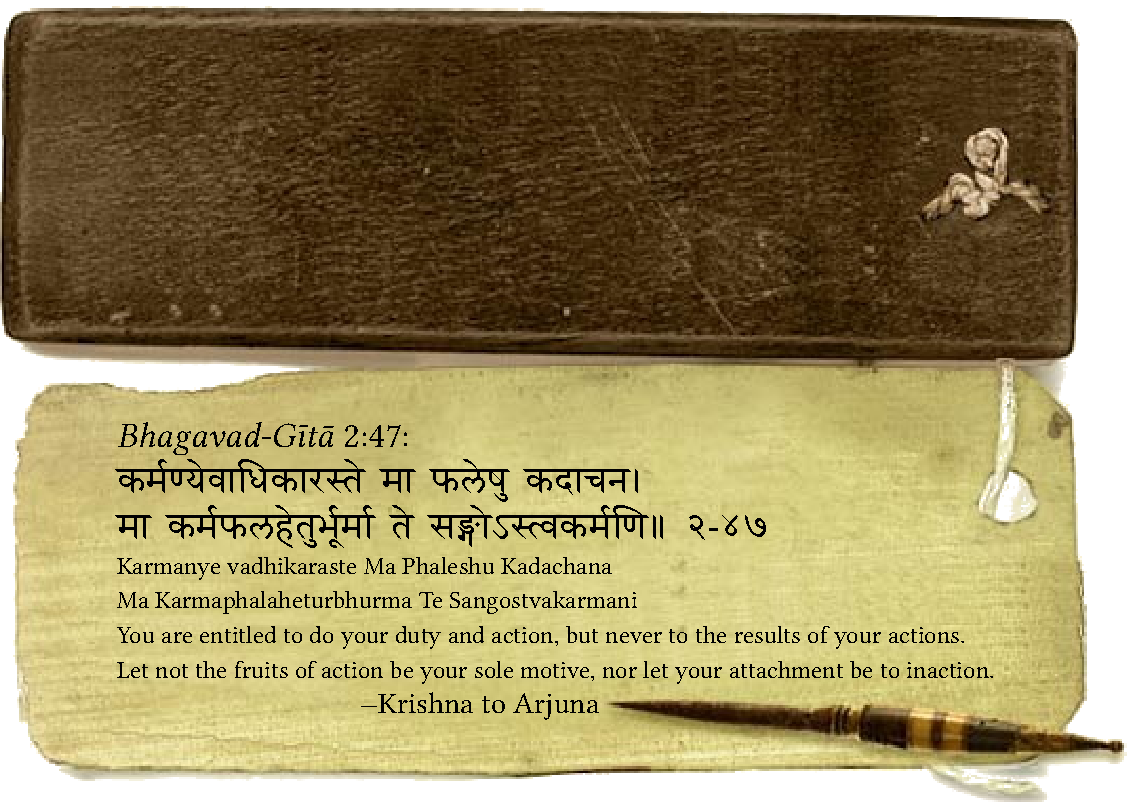
\includegraphics[width=0.85\textwidth]{narayam_sanskrit.png}
    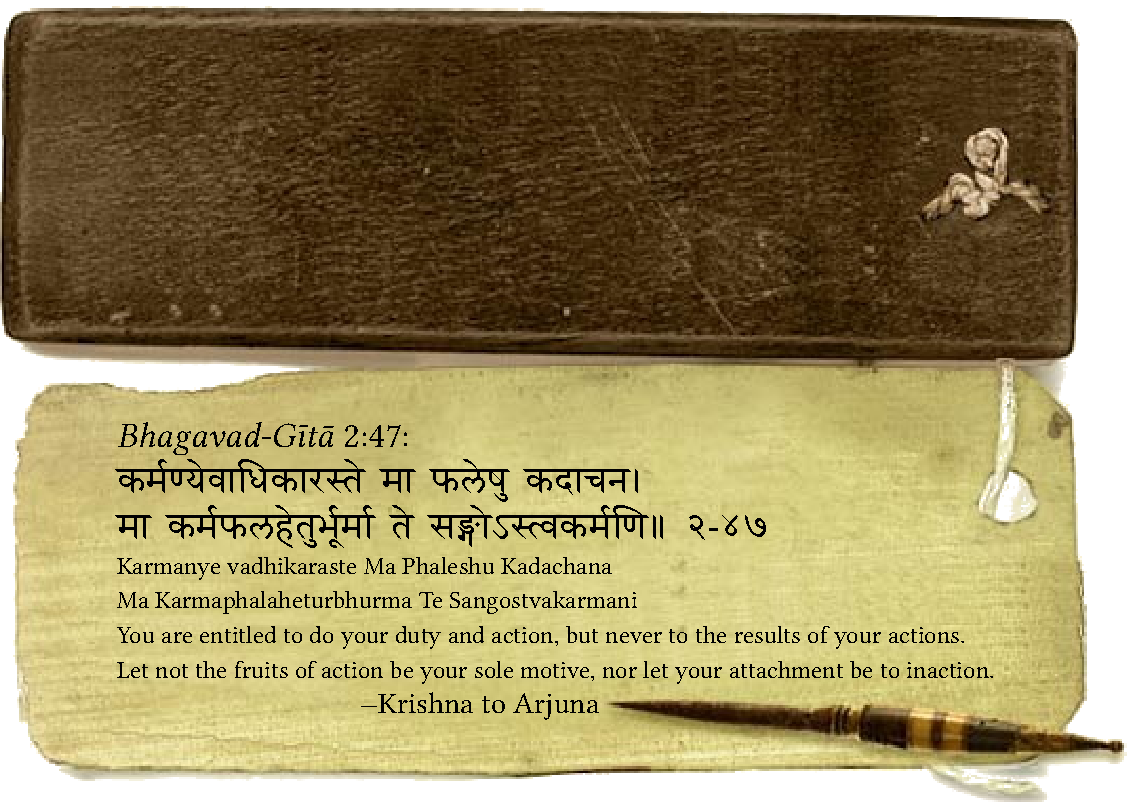
\includegraphics[width=0.85\textwidth]{narayam_sanskrit.pdf}
    \flushright{\scriptsize The image `Thaliyola.jpg' (on which the Gita verse
    is overlaid by this thesis author) was sourced from Wikimedia Commons and is licensed CC-BY-SA 2.5}

    % \pdfbookmark[chapter]{Dedication}{dedication}
\end{minipage}
\endgroup

 % -*- root: ../main.tex -*-
% !TEX root = ../main.tex
% vim:textwidth=80 fo=cqt

% \setstretch{1.16}
\setstretch{1.14125}
% \chapter*{\vspace{-1.75in}Acknowledgements\hfill} % https://latex.org/forum/viewtopic.php?t=11734
% \addcontentsline{toc}{chapter}{Acknowledgements}
\myackchapter{Acknowledgements}
\vspace*{-17mm}

% \addlines[0.5]
\addlines[1]

Obtaining a PhD has long been a dream of mine. This dream could not have come to
fruition without the support of many of my well-wishers to whom I shall remain
eternally grateful. Here, I would like to acknowledge their invaluable support
in aiding this achievement.

I wish to incorporate \emph{Sahadharmiṇī} (companion soul) and
\emph{Bandhu-Mithradhikal} (relatives and friends) into the classical quartet of
support pillars --- \emph{Matah} (mother), \emph{Pitah} (father), \emph{Guru}
(teacher), \emph{Deivam} (God) --- commonly attributed as reasons for one's
success in ancient Indian scriptures such as the Vedas, Shastras, Charitras,
Itihasas and Purāṇas. Whilst making this personal amendment, I would like to
de-emphasise any connotations of hierarchy amongst these support pillars, since
they all play equally important roles in one's life.

During these four years, the level of support accorded by my wife Parvathy Chittur
Subramanianprasad cannot be described in mere words. She voluntarily shouldered
all matters of responsibility in the family so that I could focus solely on my
research. At this prime of her youth, she has sacrificed so many material
comforts and happily lived a relatively austere life by humbly accepting the
financial constraints that are part and parcel of a student's life. In the same
vein, I owe a lot to my parents Shri~Gopalakrishnan~P.~K.\ and
Smt.~Ananthalakshmi~G. It has been ten long years since I departed Indian shores
in pursuit of higher studies. During all those years, despite ill-health and
missing my presence at home, they have always urged me to carry on and complete
my studies. Many a time, I have experienced a hopeless sense of incompleteness
due to my inability to fulfil the basic duties of a son towards his parents, the
least of which is spending quality time with them. However, my parents have
always brushed aside their physical and financial difficulties to put my success
above everything else.

% \addlines

It is needless to explain the crucial role of academic supervisors in the life
of a doctoral candidate. I~was extremely lucky to be bestowed with not just one,
but two amazing supervisors here at Imperial College London --- \mbox{Dr Gregory
J.\ Offer} and \mbox{Dr Monica Marinescu}. I~have immensely benefited from their
supervision, both from technical and personal perspectives. Even during moments
of sheer despair, my supervisors steadfastly held faith in my abilities. Their
unflinching support contributed in no small measure for this success of mine.
I~also wish to acknowledge \mbox{Dr Davide M.\ Raimondo} who served as my
unofficial supervisor and allocated months of his personal time for my research,
often well outside regular working hours. I~also wish to express my gratitude to
\mbox{Dr Gregory L.\ Plett} who has always generously offered his technical
expertise and guidance on all my research ideas. I~am thankful to \mbox{Dr Teng
Zhang} who mentored me in my initial days here and without his feedback, I~could
not have published my first journal article.

Although my interaction with them has sadly been on the wane in recent years,
I~am lucky to be a recipient of the blessings of my thatha \mbox{(Shri~Hariharan
S)} and paatti \mbox{(Smt.\ Parvathi Hariharan)}, my affectionate grandparents,
who have lived a life of humility, adhering to time-honoured traditions, whilst
seeming to have an endless reserve of love to bestow. During my childhood years,
I have been fortunate to receive a tremendous amount of affection from my
paternal grandmother, the late Smt.~Annapoorni Ammal. On this momentous
occasion, I hereby offer my \emph{pranams} to her departed soul.  I am immensely
fortunate  to have benedictions of the noble soul and towering figure, Acharyan
\mbox{Shri C R Krishna Iyer}, affectionately known as `thathanna', who has
recently attained the lotus feet of Lord Guruvayoorappa. Although I have not yet
attempted to imbibe the spiritual hints bequeathed by him, I hope to be a worthy
beneficiary of its legacy with passage of time.

My father-in-law, \mbox{Dr Subramaniaprasad C K} or CKSP/Chithappa, as he is
fondly known in our family circles, has been a father-like figure to me. From
procuring transcripts at my alma-mater at the start of my PhD journey, all the
way until providing regular feedbacks by proofreading this thesis, he has been a
strong driving force behind my success.

Members of my extended family have long been staunch supporters of my
educational aspirations. I~vividly recollect the day I~offered
\emph{namaskaarams} to Kaimal Chithappa before my first journey outside India
prior to commencing Masters' studies at Virginia Tech. \mbox{Shri~Keshava
Kaimal} has been a strong motivator and was one of the earliest in my family to
instigate a passion for engineering in me. His erudite teachings, such as as the
translation of  \enquote{Agnayeh, ithanna mamah (Oh~Agni! This is not for me;
this is for the society)} still ring in my ears and I~shall certainly strive to
rise up to such lofty ideals.

I am immensely thankful to my sister, Smt.~Radhika Balaji for constantly
cheering me up. Not for a moment has her belief in me wavered, and I~am relieved
that I~did not let her down. I~would like to express my gratitude to Smt.~Usha
Prasad whose calmness and compassion were a solace during difficult personal
times, and to Smt.~Radha Ramaswamy, whose enthusiasm has been a  buoyant
motivator. I~wish to thank Balaji Anna, Shri~Ramaswamy Krishnan Chittur (Ramesh)
and Dr~Sandeep Sangameswaran, all of whom have been more than what even brothers
could be and have always lent their support throughout.


\addlines[1]

Despite not having interacted much with her, the abilities of our beloved Manni
Ammal from Chittur remind me that one should not be carried away by their
achievements. In India, a female attending school in the pre-independence era,
particularly in a rural Kerala village, is virtually unheard of. Not only did
Manni top her high-school grades, she can reel off the Nobel-winning
\emph{Gitanjali} in fluent English, despite being hampered by the age-related
afflictions of a nonagenarian. On the same note, I bow before the vast knowledge
and humility of Shri~Ramaswamy~C.~K.\ and Smt.~Uma Sangameswaran which have
endlessly inspired me.


I would like to express my sincere gratitude to my uncles and aunts
(Shri~Kannan, Smt.~Subbalakshmi, Shri~Jayakumar, Smt.~Lalitha,  Shri~Nandakumar,
Smt.~Asha, Shri~Kaimal, Smt.~Ranjini, Shri~Dwarakanath, and Smt.~Brinda) and to
all my cousins who used to note with pride that I was the first in the family to
pursue higher studies outside India, and now the first one to complete a
doctoral degree. During  difficult times in the PhD, I am glad to have had the
cheerful support of Smt.~Remya and Smt.~Shyama, whose light-hearted approaches
to many issues is certainly worth learning from. I am thankful to Lakshmi athai,
Seetha athai and Shankar athimbere for their constant support and encouragement.
I wish to express my gratitude to Shri.~Sundar Krishnamurthy and Smt.~Anu
Sundar for all their help during the initial days to in the UK.
The next generation in the immediate family --- Arjith, Siddharth, Aditya and
little Usha kutty --- provided respite from the monotonicity of doctoral studies
through their carefree joy and innocence.

% \addlines[1]

On the technical front outside my specific research area, I would like to
acknowledge the scores of individuals who have contributed to open-source
projects for free. It is due to their efforts that much of the computational
research work in the modern era is possible. I~wish to express my admiration of
\mbox{Dr~Donald E.\ Knuth} and \mbox{Dr~Leslie Lamport} for giving us the \TeX{}
typesetting system and the \LaTeX{} macro package respectively, that immensely
helped in document authoring. I am also thankful to Bill Joy and Bram Moolenaar
for developing the \texttt{vi} and \texttt{vim} text editors, whose sheer power
eased my pain during coding and thesis writing sessions. I am thankful to the
senior contributors (David Carlisle, Ulrike Fischer, Nicola Talbot, Jonathan
Spratte to name just a few) of the TeX forum in the StackExchange family of
portals, for their personalised support and patient answers to my rather dull
questions. I also wish to tip my hat to Jorge Cham for his visceral portrayal of
life in graduate school through PhD~comics, that has never failed to put a smile
on my face.

\addlines[2]

I would like to acknowledge members of my research group (Alexander Holland,
Emma Vendola, Ian Campbell, Ian Hunt, Mei-Chin Pang, Oisin Shaw, Wasim Sarwar,
Yan Zhao, Yu~Merla to name a few) for their companionship during my studies
here. Although few and far between, the conversations in the coffee room with my
group members as well as those with other PhD students here at Imperial (James
Tebbutt, Joel Henry, Manikandan Ganapathy, Marco Da Costa Alves, Xianyan Zhou
and many others), had always lent the shared comfort of being fellow travellers
on the same journey. I am deeply touched by the gesture of Mei-Chin, who prayed
for me  in the hours leading up to the thesis submission to give me strength and
endurance. I am thankful to her for being a good friend with whom I could share
technical as well as personal challenges. I would like to thank Abhilash, Ambuj,
Anand, Arjun, Ashok, Bharath, Bibin, Divya, Elvira, Hari, Jagadees, Karthik,
Krishnan, Lakshmi, Manu, Manoj, Nagu, PK, Praveen, Ram, Remya, Sakthi, Satya,
Silby, Sita, Sreevisakh, Varsha, Vinay, Vivek, and Xavier for the camaraderie
and time-tested friendship, the fond memories of which motivated me to carry on
the  battle, even in the bleakest of times.

Last, but not the least, I would like to thank God Almighty --- the universal
driving force well beyond any specific forms of personification --- for enabling
me to complete this doctorate degree. \emph{Tathastu!} (so let it be).

\setstretch{1.348361657291667}   % golden-ratio stretch (1.2 x 1.348 = 1.618)



\setstretch{1.348361657291667}   % golden-ratio stretch (1.2 x 1.348 = 1.618)
% Thesis Abstract -----------------------------------------------------

%\begin{abstractslong}    %uncommenting this line, gives a different abstract heading
\begin{abstracts}        %this creates the heading for the abstract page
\addcontentsline{toc}{chapter}{Abstract}
Put your abstract here...

\end{abstracts}



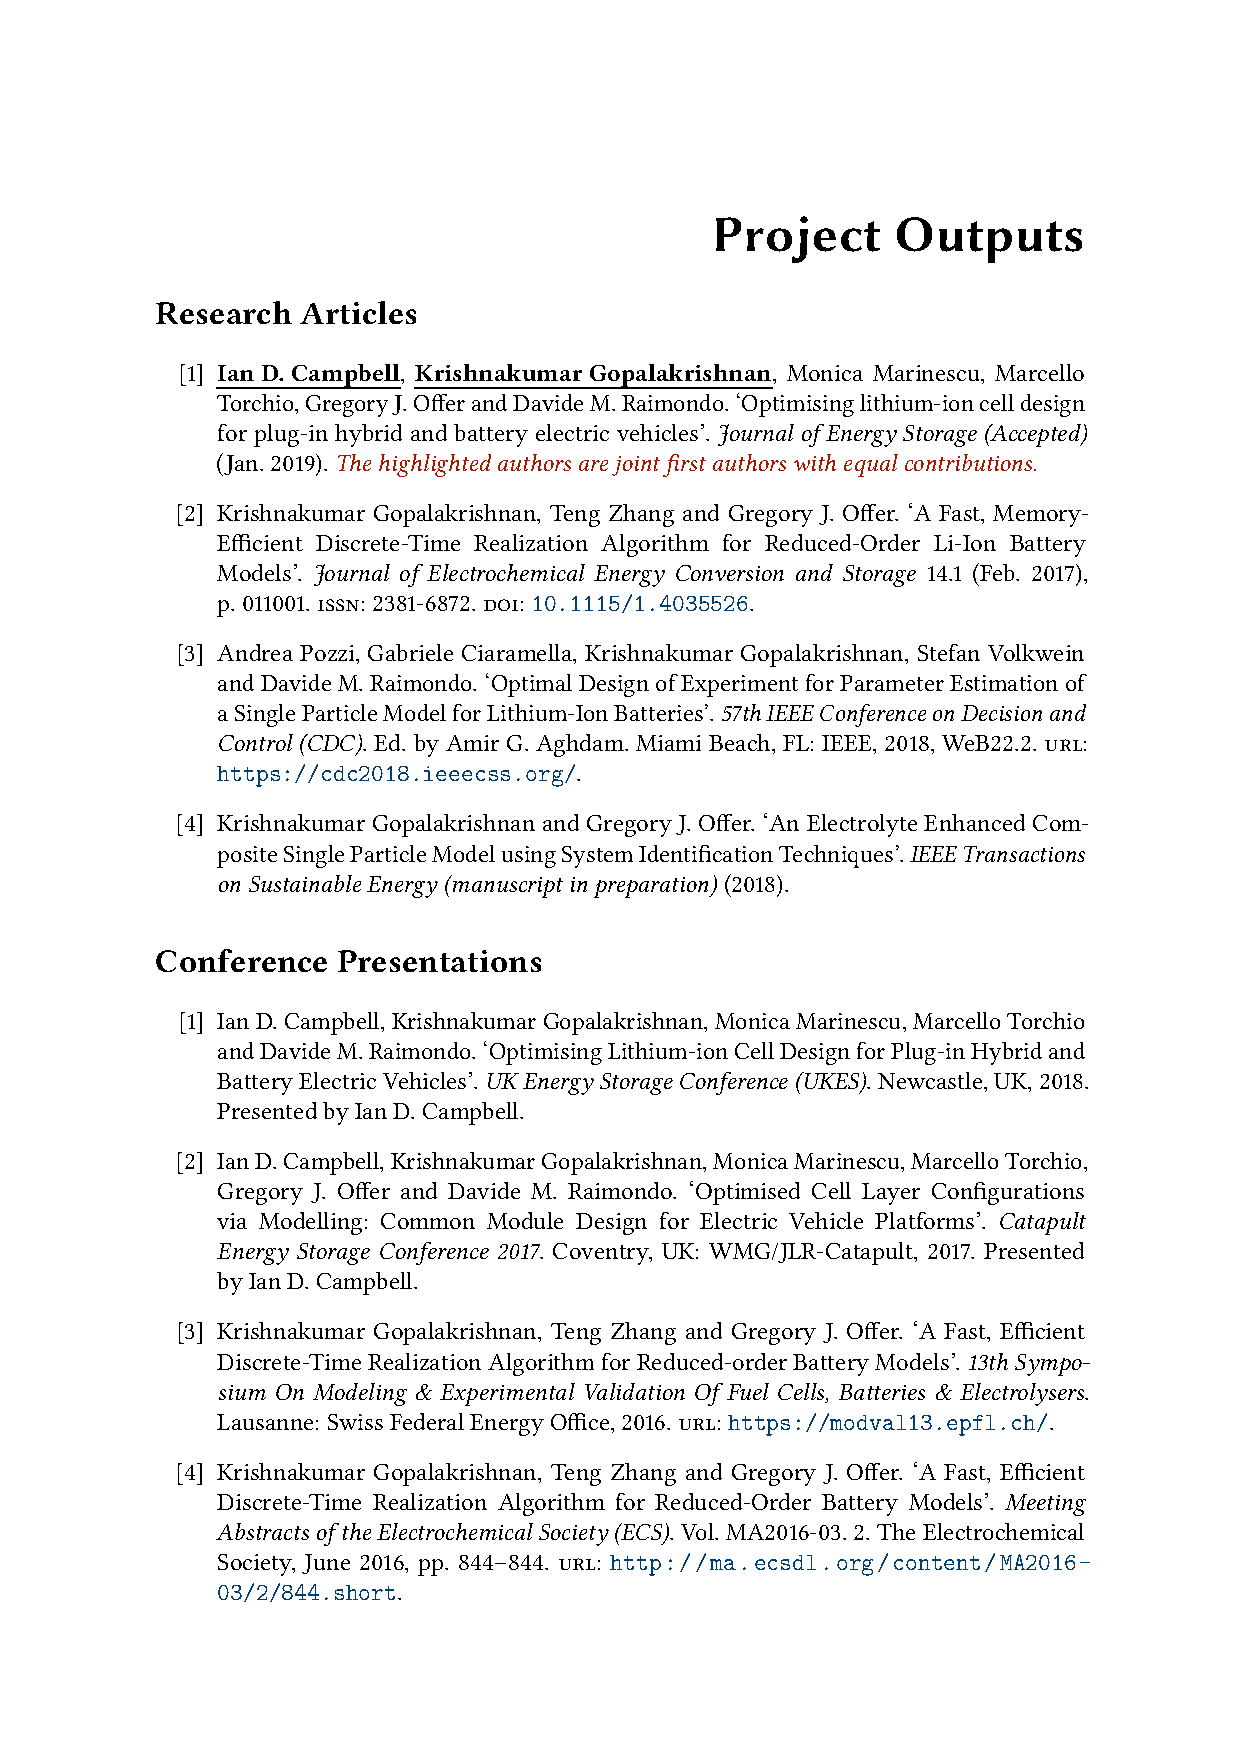
\includepdf[link, linkname=projectoutputs, addtotoc={1,chapter,0,Project outputs,projectoutputs}, pages=-, pagecommand={\thispagestyle{plain}}]{frontmatter/project_outputs.pdf}

%: ----------------- Table of contents/lof/lot/loa etc. ------------------------
\renewcommand{\baselinestretch}{0.3}\normalsize % for toc
\cleardoublepage
\glsunsetall
\microtypesetup{protrusion=false} % disables protrusion locally in the document for typesetting of toc-type matter
\pdfbookmark[chapter]{\contentsname}{toc} % \pdfbookmark[<level>]{<title>}{<dest>} with bookmark package. https://tex.stackexchange.com/questions/65544/how-to-link-table-of-contents-in-thesis-pdf
\tableofcontents
\cleardoublepage
\setstretch{1.1} % for lof
\listoffigures
\cleardoublepage
\onehalfspacing  % for lot
\listoftables
\cleardoublepage
% https://tex.stackexchange.com/questions/69184/remove-blank-page-between-list-of-figures-and-list-of-tables
{\listofalgorithms \let\clearpage\relax \addcontentsline{toc}{chapter}{List of Algorithms} \begingroup \tcblistof[\chapter*]{mypyg}{List of Program Code} \endgroup \addcontentsline{toc}{chapter}{List of Program Code}} % All of this is a hack and must be investigated properly when reusing these macros for other similar long documents
\microtypesetup{protrusion=true} % re-enables protrusion
\glsresetall
%:------------------ End of table of contents/lof/lot/loa etc.----------

% \setstretch{1.0} % for acronyms
\setstretch{1.025}
{%
\setlength{\glsdescwidth}{0.99\textwidth}
\printunsrtglossary[type=acronym, title={List of Acronyms}, nonumberlist, style=super]\label{ch:glossary}
}%
\renewcommand{\baselinestretch}{0.3}\normalsize
\printunsrtglossary[type=symbols, title={List of Symbols}, style=alttreegroup]\label{ch:symbols}


